\subsection{Descripci\'on del problema}
Este problema consiste en generar la silueta de una ciudad a partir de la representaci\'on de varios edificios que la componen.
A la entrada del algoritmo voy a tener una cantidad \textbf{N} de edificios, representados con tres valores; el comienzo, su altura y dode termina. Todos los valores son enteros positivos, en relacion a cada eje, horizontal y vertical.
A la salida voy a tener representada la silueta de la ciudad como una seguidilla de puntos que representan el contorno de los edificios que \textbf{sobresalen} del resto.
La idea esto es ocultar las partes de los edificios que quedan \textbf{dentro} de otros edificios.

\subsubsection*{Escenarios t\'ipicos}
\addcontentsline{toc}{subsubsection}{Escenarios t\'ipicos}

Las siguientes instancias son las b\'asicas a las cuales se pueden reducir todos los escenarios. La primer imagen representa a los edificios que son la entrada del algoritmo con el aditivo de los puntos marcados \footnote{Aporte realizado por un compañero del curso que lo envió a la lista de mails. Todos los créditos para \'el.} que ser\'ian la solución final. Y la segunda imagen es la ciudad representada con su silueta.

\subsubsection*{Edificio B\'asico}
\addcontentsline{toc}{subsubsection}{Edificio B\'asico}
\begin{figure}[H]
\begin{center}$
\begin{array}{cc}
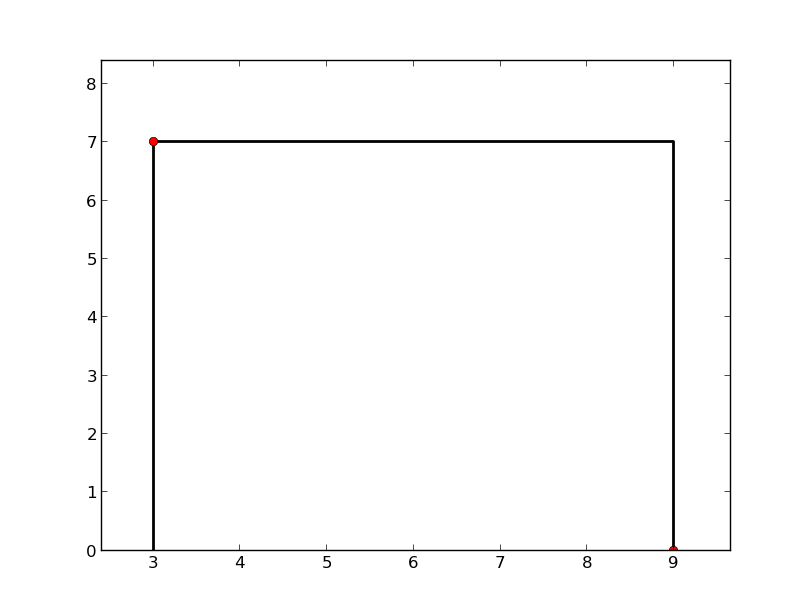
\includegraphics[scale=0.3]{./imagenes/ej2_edificio1.png}&
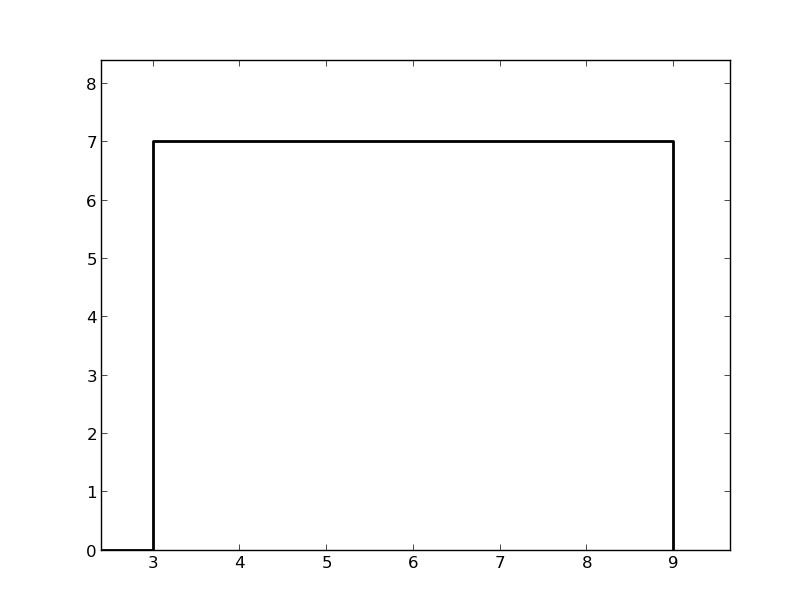
\includegraphics[scale=0.3]{./imagenes/ej2_edificio1solucion.png}
\end{array}$
\end{center}
\caption{Una ciudad con un solo edificio}
\end{figure}

\subsubsection*{Edificios Cruzados 1}
\addcontentsline{toc}{subsubsection}{Edificios Cruzados 1}
\begin{figure}[H]
\begin{center}$
\begin{array}{cc}
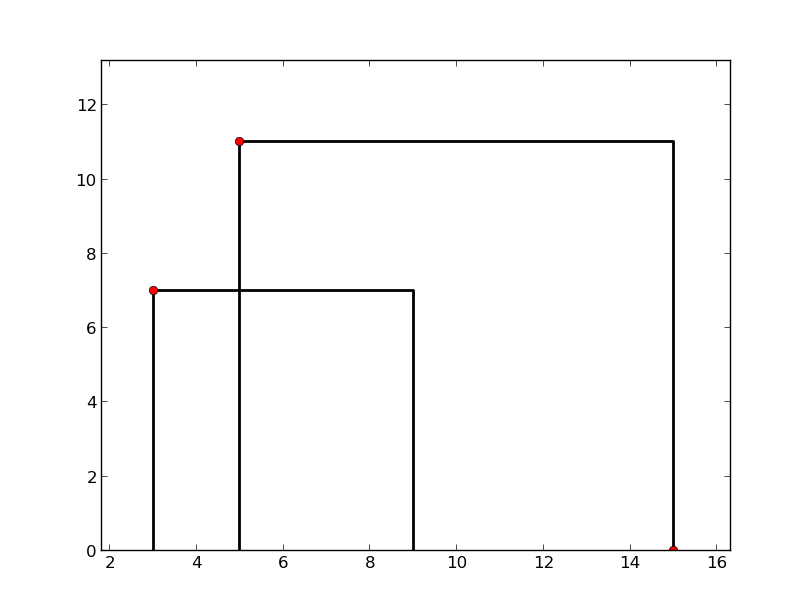
\includegraphics[scale=0.3]{./imagenes/ej2_edificio2.png}&
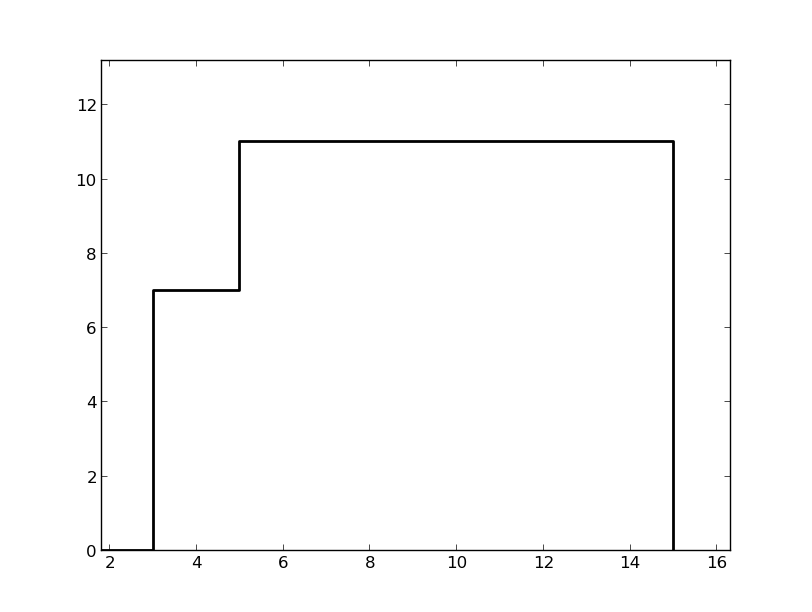
\includegraphics[scale=0.3]{./imagenes/ej2_edificio2solucion.png}
\end{array}$
\end{center}
\caption{Edificios Cruzados 1}
\end{figure}

\subsubsection*{Edificios Cruzados 2}
\addcontentsline{toc}{subsubsection}{Edificios Cruzados 2}
\begin{figure}[H]
\begin{center}$
\begin{array}{cc}
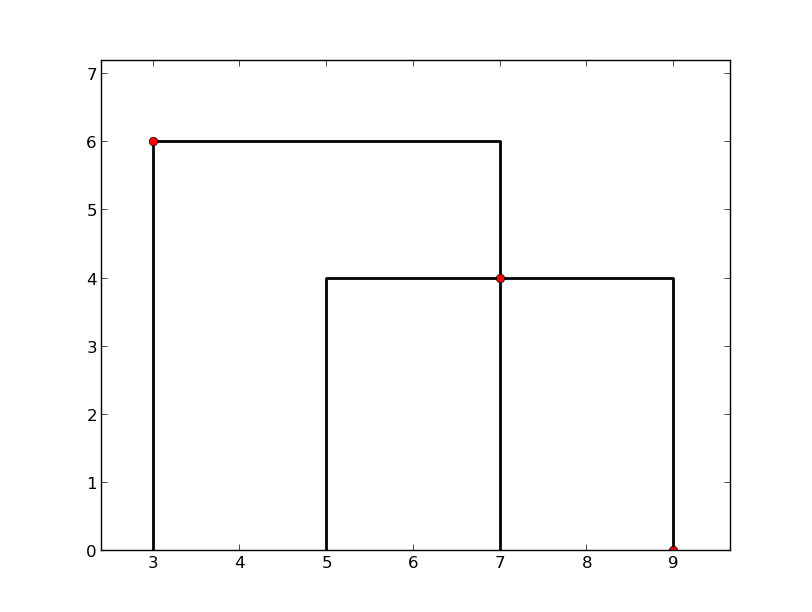
\includegraphics[scale=0.3]{./imagenes/ej2_edificio3.png}&
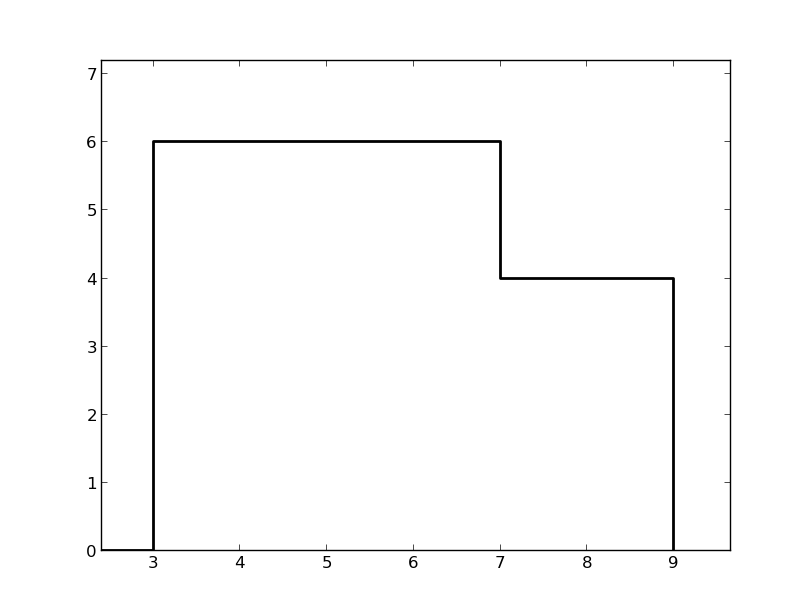
\includegraphics[scale=0.3]{./imagenes/ej2_edificio3solucion.png}
\end{array}$
\end{center}
\caption{Edificios Cruzados 2}
\end{figure}

\subsubsection*{Edificios Solapados}
\addcontentsline{toc}{subsubsection}{Edificios Solapados}
\begin{figure}[H]
\begin{center}$
\begin{array}{cc}
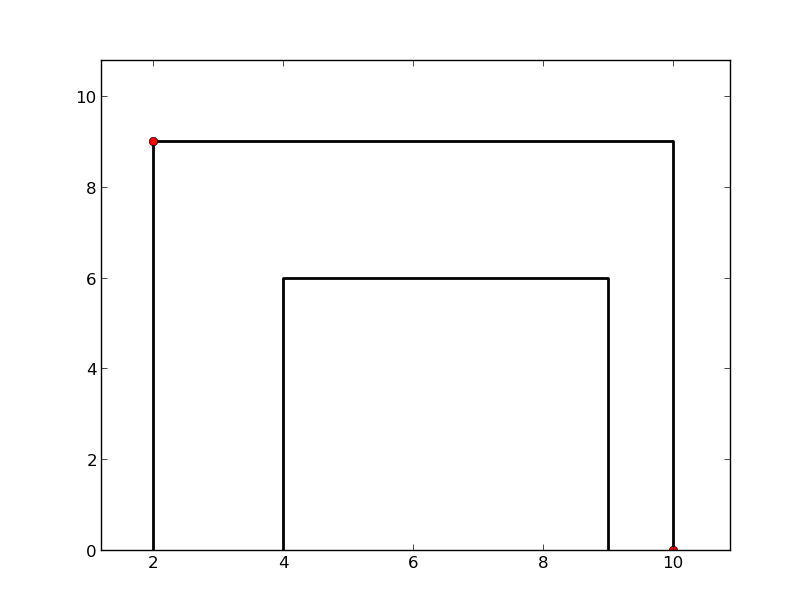
\includegraphics[scale=0.3]{./imagenes/ej2_edificio4.png}&
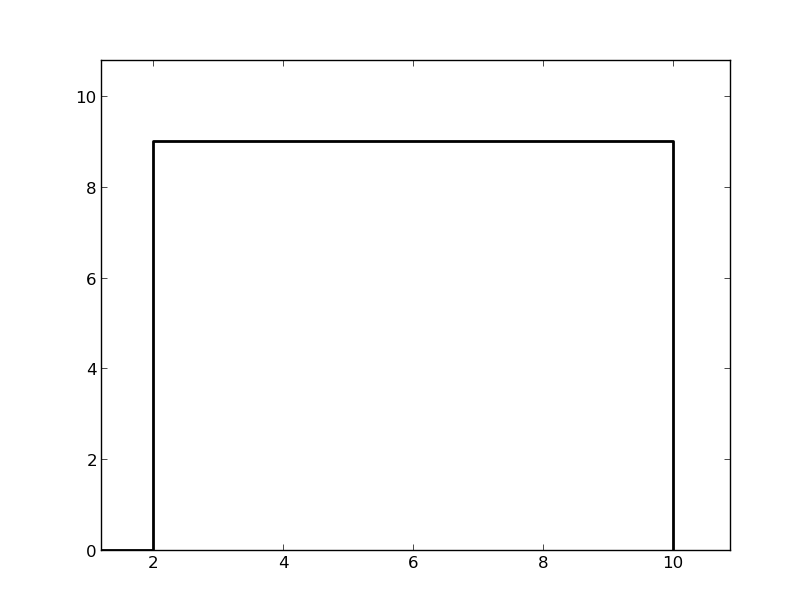
\includegraphics[scale=0.3]{./imagenes/ej2_edificio4solucion.png}
\end{array}$
\end{center}
\caption{Edificios Solapados}
\end{figure}

\subsubsection*{Edificios Contiguos}
\addcontentsline{toc}{subsubsection}{Edificios Contiguos}
\begin{figure}[H]
\begin{center}$
\begin{array}{cc}
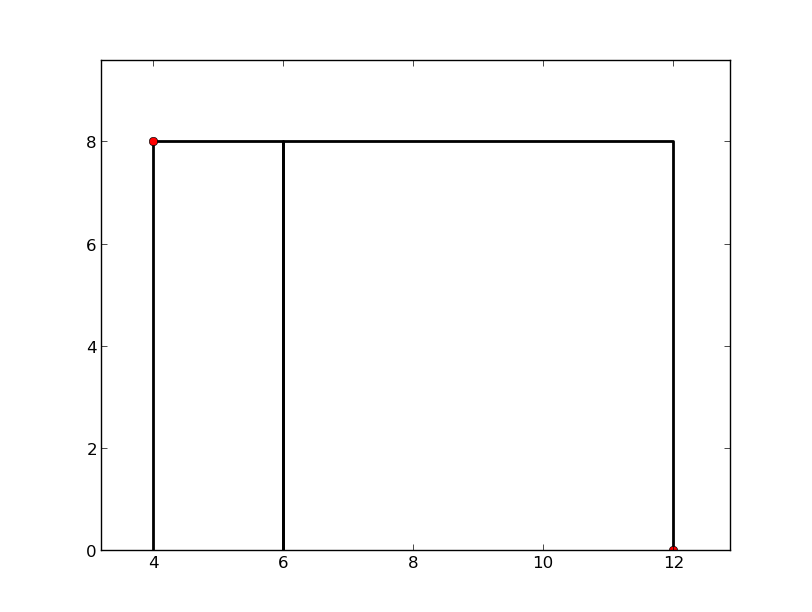
\includegraphics[scale=0.3]{./imagenes/ej2_edificio5.png}&
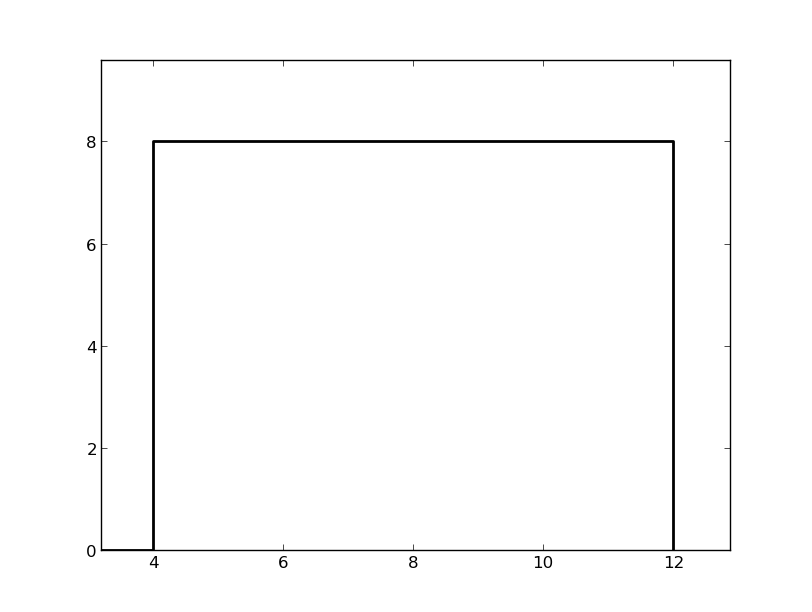
\includegraphics[scale=0.3]{./imagenes/ej2_edificio5solucion.png}
\end{array}$
\end{center}
\caption{Edificios Contiguos}
\end{figure}


\subsubsection*{Edificios Varios}
\addcontentsline{toc}{subsubsection}{Edificios Varios}
\begin{figure}[H]
\begin{center}$
\begin{array}{cc}
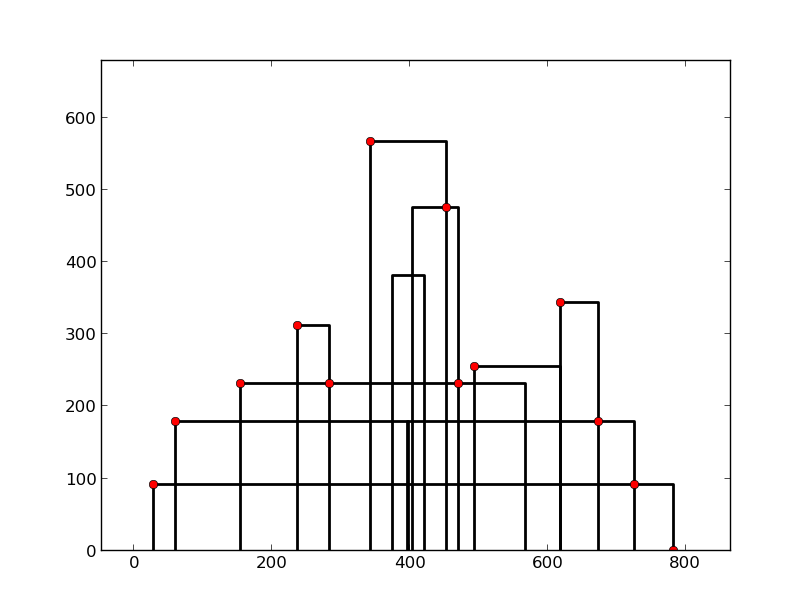
\includegraphics[scale=0.4]{./imagenes/ej2_edificio6.png}&
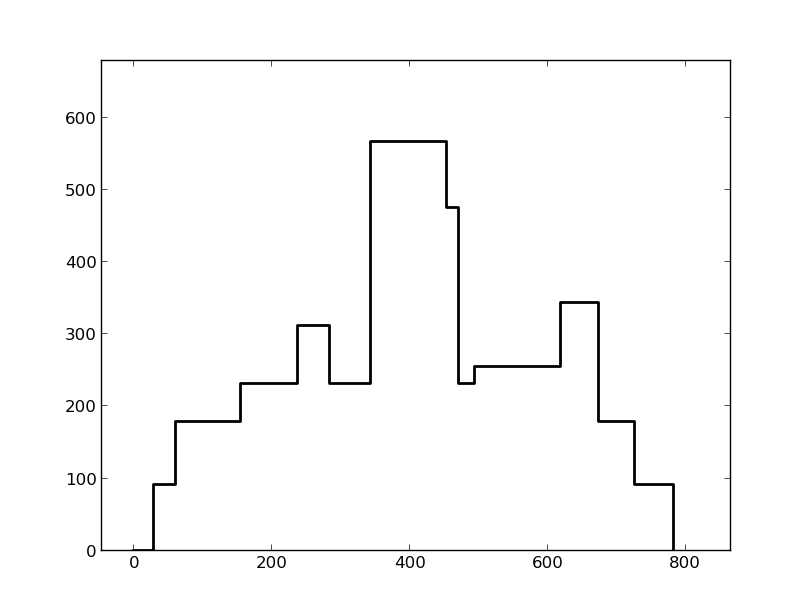
\includegraphics[scale=0.4]{./imagenes/ej2_edificio6solucion.png}
\end{array}$
\end{center}
\caption{Edificios Varios}
\end{figure}

\subsection{Resoluci\'on}
Para la resolución de este problema se optó por una estrategia simple. Vamos a generar un tipo de dato que representa un \texttt{PuntoCritico} (un punto en el eje orizontal que representa el comienzo de un edificio o su final), para luego ordenar en forma creciente todos los puntos que tiene una ciudad y analizar haciendo una barrida lineal punto a punto para luego tomar la decisi\'on de que punto (no necesariamente PuntoCritico) va a formar parte de la solución del problema.
Se decidió por esta metodología, ya que al trabajar con un tipo de dato comparable, los algoritmos de ordenamiento que se basan en comparaciones se pueden utilizar sin ningún problema.

El problema se divide en tres etapas:

\begin{enumerate}[I]
	\item Pasar nuestra entrada de N edificios a 2N PuntosCriticos, que coresponden al comienzo y final de cada edificio.
		\begin{itemize}
		\item  Se recorre linealmente la colección de edificios y se generan 2 PuntoCritico por cada uno, y \'estos se insertan en una colección de PuntosCriticos.
		\end{itemize}
	\item Ordenar nuestro nuevo arreglo de 2N PuntosCriticos para luego analizar en orden ascendente.
		\begin{itemize}
		\item  Se ordena la colecci\'on \footnote{C++ reference \url{http://www.cplusplus.com/reference/algorithm/sort/}} donde el orden está definido por:  
			\begin{itemize}
				\item Posici\'on del edificio
				\item Punto de apertura $<$ Punto de clausura
				\item Altura del edificio)
			\end{itemize}
		\end{itemize}
	\item Volver a recorrer nuestro arreglo haciendo una barrida lineal por los elementos y en cada paso tomar la decision de si tengo que agregar algun punto a la soluci\'on.
	\begin{itemize}
		\item  Al recorre la colección de PuntosCriticos, Cuando es un punto de comienzo se inserta en un \texttt{multimap} \footnote{C++ reference \url{http://www.cplusplus.com/reference/map/multimap/}}  un elemento con esa altura, cuando es un pundo de finalizaci\'on de un edificio se lo saca del \texttt{multimap} (esto es para mantener una estructura que nos ayuda a decidir que puntos pertenecen a la soluci\'on del problema).
		\end{itemize}
\end{enumerate}

No está demás aclarar que un edificio se transforma en 2 PuntoCritico:
	\begin{itemize}
		\item Apertura del edificio en la posición x, hasta una altura y
		\item Cierre del edificio en la posición x, desde la altura y
	\end{itemize}

Esto es importante ya que primero establezco un orden en el cual voy a analizar los puntos de apertura y luego los de clausura de edificios. Porque al abrir un edificio, \'este continúa siendo relevante, ya que al cerrar cualquier edificio tengo que considerar el punto al cual baja la silueta de la ciudad (el edificio más alto abierto en ese momento). La dinámica es ir abriendo y cerrando edificios cada vez que analizo un PuntoCritico de apertura o clausura, mientras considero si agrego alg\'un punto a la solución final o no.

Al tenerlos ordenados, no solo por posición, sino por tipo de PuntoCritico (Apertura/Clausura) me aseguro siempre \textbf{ABRIR} edificios antes de \textbf{CERRARLOS}. Cuando es un PuntoCritico de Apertura el que analizo lo inserto inmediatamente como edificio abierto, ya que por m\'as que en ese momento pueda que no sea relevante, por quedar oculto por un edificio más alto, en un próximo paso su altura puede intervenir en la solución final.
Y cuando es un PuntoCritico de Clausura lo cierro inmediatamente pues este edificio no interviene más en la resolución del algoritmo.

Voy a analizar en orden creciente por posici\'on de los PuntoCritico desde el edificio que comienza primero hasta el edificio que termina último.
En cada iteración tengo referencia al nivel actual de la ciudad, que comienza en 0 y se actualiza aumentando por cada PuntoCritico de apertura que incremente el nivel actual y disminuyendo por cada PuntoCritico de Clausura que corresponda al edificio abierto que estoy cerrando (porque me topé con su punto crítico de clausura) hasta el nivel que corresponda.

PuntoCritico de Apertura
\begin{itemize}
		\item Al encontrar un PuntoCrito de apertura agrego un edificio abierto que corresponde a la altura del punto cr\'itico
		\item Se puede dar que varios edificios compartan el origen (posicion en donde comienza), con lo cual avanzo hasta el PuntoCritico de igual posicion y tipo, pero mayor altura. Al estar en orden avanzo hasta encontrar uno de distinta posicion y/o tipo(con lo cual el inmediato anterior es el de mayor altura de los que comparte posicion y tipo).
			\begin{itemize}
				\item Si la altura del PC de apertura es mayor al nivel actual de la ciudad entonces este punto cr\'itico va en la soluci\'on del problema y el nivel actual de la ciudad pasa a ser la altura del mismo
				\item Si no, no es considerado en la solución, pero s\'i queda como edificio abierto para futuras consideraciones
			\end{itemize}
\end{itemize}

PuntoCritico de Clausura
\begin{itemize}
	\item Al encontrar un PuntoCrito de clausura, cierro un edificio abierto que corresponde a la altura del punto cr\'itico, con lo cual este valor ya no está en consideración a la hora de saber el máximo edificio abierto
		\begin{itemize}
			\item Si la altura no es igual al nivel actual de mi ciudad (es estrictamente menor pues si fuera mayor abr\'ia un edificio abierto de esta altura y el nivel actual ser\'ia ese) ese punto queda excluido de la solución, ya que es un punto está dentro de algún edificio abierto
			\begin{itemize}
				\item Si la altura es igual al nivel actual de mi ciudad y el edificio máximo abierto (no me considero a mi mismo, pues ya cerr\'e el edificio correspondiente a mi) es menor al nivel acual, implica que debo bajar desde el nivel actual hasta el nivel del máximo edificio abierto, con lo cual a la solución se le agrega un punto que tiene la posición de clausura del PuntoCritico y la altura del máximo edificio abierto.
				\item De lo contrario quiere decir que hay un edificio de la misma altura (mayor nunca podría ser con instancias válidas de entrada) abierto y por lo tanto este PC tampoco se considera parte de la solución.
			\end{itemize}
		\end{itemize}
\end{itemize}

Con todas estas consideraciones, todos los escenarios planteados en el principio están cubiertos, con lo cual cualquier instancia de entrada se reduce a alguna situación de las primeras mencionadas y se resuelven satisfactoriamente en todos los casos.


\subsection{Demostraci\'on de la resoluci\'on}


\subsection{Complejidad del algoritmo}


\subsection{C\'odigo Relevante}

No se consideró relevante ni la conversión de estructuras, ni el ordenamiento de los elementos por ser funciones básicas y/o implementadas en librerias de C++.

El código interesante para la resolución de este problema es aquel que recorre los PuntoCriticos en orden y decide si pertenecen o no a la solución del problema.

No se consideró relevante ni la conversión de estructuras, ni el ordenamiento de los elementos por ser funciones básicas y/o implementadas en librerias de C++.

El código interesante para la resolución de este problema es aquel que recorre los puntos críticos en orden y agrega puntos a la solución del problema.


\lstset{language=C++,
                basicstyle=\ttfamily\footnotesize,
                keywordstyle=\color{blue}\ttfamily,
                stringstyle=\color{red}\ttfamily,
                commentstyle=\color{green}\ttfamily,
                morecomment=[l][\color{magenta}]{\#},
                breaklines=true
}
\begin{lstlisting}
typedef std::multimap<int,PuntoCritico> MapAlturas;
typedef std::vector<int> Ciudad;

struct PuntoCritico{
	PuntoCritico(bool s, Edificio& e){
		edificio = &e;
		sube = s;
		altura = e.altura;
		if (s){
			posicion = e.comienzo;
		} else {
			posicion = e.fin;
		}
	}
	bool sube;
	int altura, posicion;
	Edificio* edificio;
};

//El orden esta establecido por: Posicion,Sube o Baja, Altura
struct orden_PuntoCritico{
	bool operator()(const PuntoCritico& a, const PuntoCritico& b) const{
		if(a.posicion == b.posicion){
			if (a.sube == b.sube){
				return a.altura < b.altura;
			} else {
				return a.sube > b.sube;
			}
		} else {
			return a.posicion < b.posicion;
		}
	};
};

std::vector<PuntoCritico> puntos;
MapAlturas edificiosAbiertos;

std::vector<PuntoCritico>::iterator itPuntos = puntos.begin();
	//Recorro los 2N elementos
	for(;itPuntos!=puntos.end();++itPuntos){
		if (itPuntos->sube){
		//Si es un punto de comienzo de un edificio
			//agregar al mapa el edificio abierto
			edificiosAbiertos.insert(make_pair(itPuntos->altura,*itPuntos));
			std::vector<PuntoCritico>::iterator itCopy = itPuntos;
 			if(*(++itCopy) == *itPuntos){
 			//Si no es el mas alto de los edificios que empiezan en la misma posicion.	
				continue;
			} else if (itPuntos->altura > nivelActual){
			//Si el nivel de este edificio supera al nivel actual del recorrido
				//Lo inserto en la solucion
				ciudad->push_back(itPuntos->posicion);
				ciudad->push_back(itPuntos->altura);
				//Actualizo el nivel actual
				nivelActual = itPuntos->altura;
			}
		} else {
		//Si es un punto de cierre de un edificio
			//Sacar del mapa el edificio que estoy cerrando
			MapAlturas::iterator it = edificiosAbiertos.find(itPuntos->altura);
			edificiosAbiertos.erase (it);
			//Consigo el maximo edificio abierto
			MapAlturas::iterator itEdificiosAbiertos = --edificiosAbiertos.end();
			int alturaMaximoEdificio = (*itEdificiosAbiertos).first;
			if(itPuntos->altura == nivelActual && alturaMaximoEdificio < itPuntos->altura){
			//Si estoy bajando desde el edificio que esta abierto y no hay ninguno del mismo tamano
				//Inserto el punto de bajada hasta la posicion del maximo abierto
				ciudad->push_back(itPuntos->posicion);
				ciudad->push_back(alturaMaximoEdificio);
				//Actualizo el nivel actual
				nivelActual = alturaMaximoEdificio;
			}
		}
	}
\end{lstlisting}

\end{lstlisting}

\subsection{Casos de prueba}

\subsection{Performance}
